\appendix

\part*{ANEXOS}
\addcontentsline{toc}{part}{ANEXOS}
\refstepcounter{part} 

\chapter{Código do \emph{HTML} da Parte 1}
\label{appendix:a}

\begin{longlisting}
	\inputminted{html}{testes/res_html.html}
	\caption{Resultado do \emph{output} da aplicação do filtro na Parte 1}
	\label{listing:a}
\end{longlisting}


\chapter{Código dos ficheiros do \hologo{BibTeX} para testes}
\label{appendix:a1}

\begin{longlisting}
	\inputminted{tex}{testes/ex3.bib}
	\caption{Ficheiro fonte \hologo{BibTeX} para testes --- parte 2 e 3}
	\label{listing:a1}
\end{longlisting}

\begin{longlisting}
	\inputminted{tex}{testes/ex4.bib}
	\caption{Ficheiro fonte \hologo{BibTeX} para testes --- parte 4}
	\label{listing:a2}
\end{longlisting}

\chapter{Resultado da Parte 2}
\label{appendix:b}

\begin{longlisting}
	\inputminted{tex}{testes/resNorm.bib}
	\caption{Resultado do \emph{output} da aplicação do filtro na Parte 2}

	\label{listing:b}
\end{longlisting}

\chapter{Resultado da Parte 3}
\label{appendix:c}

\begin{longlisting}
	\inputminted{tex}{testes/res_pretty_printing.txt}
	\caption{Resultado do \emph{output} da aplicação do filtro na Parte 3}

	\label{listing:c}
\end{longlisting}

\chapter{Resultado da Parte 4}
\label{appendix:d1}
\begin{longlisting}
	\inputminted{tex}{testes/res_dot.dot}
	\caption{Resultado do \emph{output} da aplicação do filtro na Parte 3}

	\label{listing:d1}
\end{longlisting}
\newpage

\begin{figure}[hbtp]
	\centering
  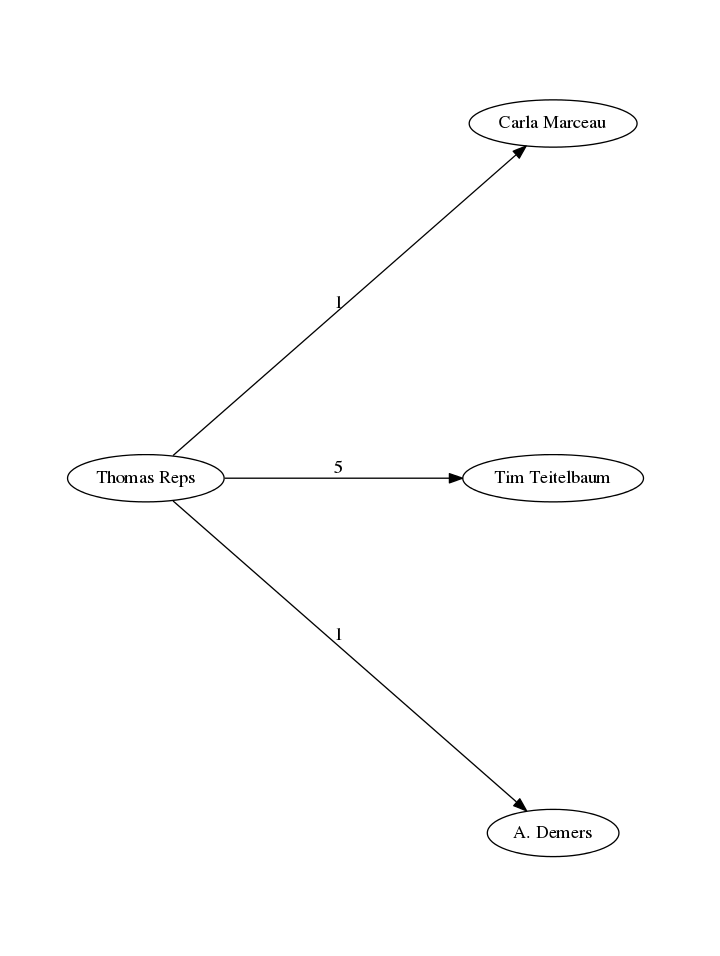
\includegraphics[scale=0.5]{testes/out.png}
	\caption{Grafo Resultante da aplicação do filtro da Parte 4}
	\label{fig:d1}
\end{figure}









